%===================================================================================
% JORNADA CIENTÍFICA ESTUDIANTIL - MATCOM, UH
%===================================================================================
% Esta plantilla ha sido diseñada para ser usada en los artículos de la
% Jornada Científica Estudiantil de MatCom.
%
% Por favor, siga las instrucciones de esta plantilla y rellene en las secciones
% correspondientes.
%
% NOTA: Necesitará el archivo 'jcematcom.sty' en la misma carpeta donde esté este
%       archivo para poder utilizar esta plantila.
%===================================================================================



%===================================================================================
% PREÁMBULO
%-----------------------------------------------------------------------------------
\documentclass[a4paper,10pt,twocolumn]{article}

%===================================================================================
% Paquetes
%-----------------------------------------------------------------------------------
\usepackage{amsmath}
\usepackage{amsfonts}
\usepackage{amssymb}
\usepackage{jcematcom}
\usepackage[utf8]{inputenc}
\usepackage{listings}
\usepackage[pdftex]{hyperref}
\usepackage{caption}
\usepackage{subcaption}
\usepackage{siunitx}
%-----------------------------------------------------------------------------------
% Configuración
%-----------------------------------------------------------------------------------
\hypersetup{colorlinks,%
	    citecolor=black,%
	    filecolor=black,%
	    linkcolor=black,%
	    urlcolor=blue}

%===================================================================================



%===================================================================================
% Presentacion
%-----------------------------------------------------------------------------------
% Título
%-----------------------------------------------------------------------------------
\title{Un enfoque hacia la Miopía. Análisis Exploratorio de Datos.}

%-----------------------------------------------------------------------------------
% Autores
%-----------------------------------------------------------------------------------
\author{\\
\name Jackson Vera Pineda \email \href{mailto:jacksonverapineda@gmail.com}{jacksonverapineda@gmail.com}
	\\ \addr Grupo C312 \AND
\name Kevin Manzano Rodríguez \email \href{mailto:kevinmanzano020610@gmail.com}{kevinmanzano020610@gmail.com}
  \\ \addr Grupo C312 \AND
  \name Roger Fuentes Rodríguez \email \href{mailto:a.dos@lab.matcom.uh.cu}{a.dos@lab.matcom.uh.cu}
  \\ \addr Grupo C312
  }

%-----------------------------------------------------------------------------------
% Tutores
%-----------------------------------------------------------------------------------
\tutors{\\
Dr. Tutor Uno, \emph{Centro} }

%-----------------------------------------------------------------------------------
% Headings
%-----------------------------------------------------------------------------------
\jcematcomheading{\the\year}{1-\pageref{end}}{Vera J., Manzano K. Fuentes R.}

%-----------------------------------------------------------------------------------
\ShortHeadings{Miopía, Análisis Exploratorio de Datos}{Autores}
%===================================================================================



%===================================================================================
% DOCUMENTO
%-----------------------------------------------------------------------------------
\begin{document}

%-----------------------------------------------------------------------------------
% NO BORRAR ESTA LINEA!
%-----------------------------------------------------------------------------------
\twocolumn[
%-----------------------------------------------------------------------------------

\maketitle

%===================================================================================
% Resumen y Abstract
%-----------------------------------------------------------------------------------
\selectlanguage{spanish} % Para producir el documento en Español

%-----------------------------------------------------------------------------------
% Resumen en Español
%-----------------------------------------------------------------------------------
%\begin{abstract}
%
%	El resumen en español debe constar de $100$ a $200$ palabras y presentar de forma
%	clara y concisa el contenido fundamental del artículo.
%
%\end{abstract}
%
%%-----------------------------------------------------------------------------------
%% English Abstract
%%-----------------------------------------------------------------------------------
%\vspace{0.5cm}
%
%\begin{enabstract}
%
%  The English abstract must have have $100$ to $200$ words, and present 
%  the essentials of the article content in a clear and concise form.
%
%\end{enabstract}

%-----------------------------------------------------------------------------------
% Palabras clave
%-----------------------------------------------------------------------------------
\begin{keywords}
	Separadas,
	Por,
	Comas.
\end{keywords}

%-----------------------------------------------------------------------------------
% Temas
%-----------------------------------------------------------------------------------
\begin{topics}
	Tema, Subtema.
\end{topics}


%-----------------------------------------------------------------------------------
% NO BORRAR ESTAS LINEAS!
%-----------------------------------------------------------------------------------
\vspace{0.8cm}
]
%-----------------------------------------------------------------------------------


%===================================================================================

%===================================================================================
% Introducción
%-----------------------------------------------------------------------------------
\section{Introducción}\label{sec:intro}
%-----------------------------------------------------------------------------------
		La miopía es una enfermedad de la refracción del ojo en el cual los rayos de luz paralelos convergen en un punto focal situado delante de la retina, en lugar de converger en la misma; es lo contrario de la hipermetropía, en la que los rayos de luz llegan a la retina antes de converger \cite{semi}. Afectando (la miopía) mayormente la visón lejana.
		
		Entre los síntomas de esta condición pueden presentarse: visión borrosa en objetos que están lejos; necesidad de estremecer los ojos para ver con claridad; dolores de cabeza, y fatiga ocular. En niños, estos indicadores pueden afectar el comportamiento provocando, quizás, estremecimiento de los ojos constantemente, dificultad para notar objetos alejados, parpadeo y frotamiento frecuente de los ojos, necesidad de posicionarse cerca de la televisión u otros dispositivos.

		Existen factores que frecuentemente se asocian con un alto riesgo de aparición de la enfermedad como son la herencia genética, realizar actividades prolongadas que requieran visión de cerca, más aún si estas actividades son frente a pantallas, y poca exposición a exteriores (luz natural y recreación al aire libre).

		El presente artículo propone realizar un Análisis Exploratorio a un conjunto de datos del Estudio Longitudinal de Miopía de Orinda (OLSM por sus siglas en inglés) en California, Estados Unidos, para desarrollar un perfil predictivo de la miopía a edades tempranas. Se evaluaron 618 niños de 5 a 9 años, inscritos en el estudio.

%===================================================================================
%En un estudio que incluyó a 5,742 niños, se concluyo que el promedio de Longitud Axial (AL) era de 23.7 mm (rango: 18.3 mm a 30.4 mm).


%===================================================================================
% Desarrollo
%-----------------------------------------------------------------------------------
\section{Desarrollo}\label{sec:dev}
%-----------------------------------------------------------------------------------
%  En esta sección (o secciones) incluya el contenido fundamental del artículo.
%  No es necesario tener una sección nombrada \emph{Desarrollo}, por el contrario,
%  nombre las secciones según el contenido que tratan.
	  \subsection{Sobre los datos}\label{sub:data}
  
	Los datos fueron recuperados de Kaggle \cite{kaggle}. Las mediciones se realizaron al ojo derecho de cada individuo por tanto, cada fila es independiente a las otras. Los datos fueron recolectados de forma longitudinal, es decir, se realizó un seguimiento a cada sujeto del estudio por varios años, y en el conjunto actual se presenta la última revisión, como se especifica en el estudio por Zadnik K. \cite{zadnikpredictors}
  
 	\begin{figure*}[ht!]%
  		\begin{center}
	  		\begin{tabular}{lS[table-format=3.2]@{\space$\, \pm \,$}S[table-format=2.2]SS}
	  			\hline
	  			\multicolumn{1}{c}{\textbf{Variables}} & \multicolumn{2}{c}{\textbf{Media $\pm$ SD}} & \multicolumn{1}{c}{\textbf{Mínimo}} & \multicolumn{1}{c}{\textbf{Máximo}}\\
	  			\hline
	  			Edad & 6.30 & 0.71	& 5 & 9 \\ 
	  			Equivalente Esférico de Refracción 	& 0.80 & 0.63 & -0.70 & 4.37 \\ 
	  			Longitud Axial & 22.50 & 0.68 & 19.90 & 24.56 \\ 
	  			Profundidad de la Cámara Anterior  & 3.58 &  0.23 & 2.77 & 4.25 \\ 
	  			Grosor del Critalino & 3.54	& 0.15 & 2.96 &	4.11 \\ 
	  			Produndidad de la Cámara Vítrea & 15.38	& 0.66 & 13.38 & 17.30 \\ 
%	  			Tiempo al aire libre &	11.95 & 7.97 & 0 & 45 \\ 
%	  			Tiempo de Lectura recreativa & 2.80 & 3.07 & 0 & 20 \\
%	  			Tiempo en Computadora & 2.10 & 3.05 & 0 & 30 \\
%	  			Tiempo de estudio & 1.49 & 2.22 & 0 & 15 \\
%	  			Tiempo viendo televisión & 8.95 & 5.72 & 0 & 31 \\
%	  			Compuesto de act & 22.01 & 26.03 & 2 & 101 \\ 
	  			\hline
	  		\end{tabular}
  			\caption{ Resumen descriptivo de las variables \label{table:1}}
  	\end{center}
  \end{figure*}
  
  \subsection{Variables}\label{sub:variables}
  	  A continuacion se presentan las variables recuperadas del conjunto de datos más relevantes para el presente análisis, y, en la Tabla \ref{table:1}, se muestra un resumen descriptivo de cada una en la muestra :
  	\begin{description}
  
%  	\item \texttt{STUDYYEAR}: Año en el que se realizó la medición.
  	\item [\texttt{MYOPIC}]: Variable booleana 0 si el sujeto desarrollara miopía en los siguientes 5 años o no
  	\item [\texttt{AGE}]: La Edad del sujeto (de 5 a 9 años)
%  	\item \texttt{GENDER}: Género del sujeto 0 Femenino 1 Masculino,
  	\item [\texttt{SPHEQ}]: Equivalente Esférico de la Refracción ( Spherical Equivalent Refraction) es una estimación del error refractivo de tus ojos.
  	\item [\texttt{AL}]: La Longitud Axial se refiere a la distancia entre la parte posterior y la parte delantera del ojo   (Medición en milímetros mm).
  	\item [\texttt{ACD}]: La Profundidad de la Cámara Anterior (Anterior Chamber Depth) se refiere a la distancia entre la superficie anterior de la córnea y la superficie anterior del cristalino (Medición en milímetros).
  	\item [\texttt{LT}]: El grosor del cristalino (Medición en milímetros mm) rango de 20.48-35.05 mm.
%  	Cambios con la Longitud Axial (AL): El LT no cambia de manera lineal con la AL. En ojos cortos, el LT aumenta a medida que la AL aumenta. Sin embargo, en ojos normales o moderadamente miopes, disminuye con una AL más larga. Curiosamente, en ojos altamente miopes, vuelve a aumentar con una AL mayor. El LT máximo se encuentra en el grupo de AL de 20.01–22 mm.
%  	El LT se correlaciona negativamente con la ACD.
  	\item [\texttt{VCD}]: La Profundidad de la Cámara Vítrea (Vitreous Chamber Depth, en inglés) en oftalmología se refiere a la distancia entre la parte posterior del cristalino y la retina.
%  	En pacientes en edad pediátrica existe una correlacion débil directa, pero no puede asegurarse puesto que puede depender de otros factores.
%  	\item [\texttt{SPORTHR}]: Tiempo de Recreación al aire libre (Horas por Semana)
%	\item [\texttt{READHR}]: Tiempo de Lectura recreativa (Horas por Semana)
%  	\item [\texttt{COMPHR}]: Tiempo Activo en Computadora o consolas (Horas por Semana).
% 	\item [\texttt{STUDYHR}]: Tiempo de estudio (Horas por Semana).
%  	\item [\texttt{TVHR}]: Tiempo viendo televisión (Horas por Semana).
%  	\item [\texttt{DIOPTERHR}]: Compuesto de actividades cercanas al trabajo (horas/semana).
  	\item [\texttt{MOMMY}]: Se refiere a si la madre es miope 0 negativo, 1 positivo.
  	\item [\texttt{DADMY}]: Se refiere a si el padre es miope 0 negativo, 1 positivo.
  	
  	%
  \end{description}
  
  

  

%%-----------------------------------------------------------------------------------
%	\subsection{Organización del Documento}\label{sub:results}
%%-----------------------------------------------------------------------------------
%		Puede agregar secciones y subsecciones según sea necesario para organizar
%		de manera más coherente su artículo. Tenga en cuenta que un documento más
%		plano es más fácil de navegar y entender, pero las subsecciones relacionadas
%		deberían estar agrupadas en una sección común.
%		
%		
%		Los nombres de las secciones deben ir en mayúsculas, excepto para las
%		preposiciones, conjunciones, y otros vocablos auxiliares.
%
%		Empiece un nuevo párrafo cada vez que vaya a comenzar una idea nueva.
%		
%-----------------------------------------------------------------------------------
\subsection{Pruebas de Hipótesis}\label{sub:hiptesting}
%-----------------------------------------------------------------------------------
	El uso de datos de longitud axial (\emph{AL}) es valioso tanto para determinar el riesgo para la salud ocular, como para juzgar la eficacia de un tratamiento para el control de la miopía. Varios estudios han demostrado la correlación entre la biometría ocular, especialmente la AL, con los errores refractivos: se encontró que el diámetro corneal, el Equivalente Esférico de la Refracción (SPHEQ) y la profundidad de la cámara Vítrea (ACD) afectaban los parámetros de la AL. Estas correlaciones pueden distinguirse en la Figura \ref{fig:4}.
	
	Cabe destacar en la Figura \ref{fig:4} cómo el SPHEQ a priori parece ser un elemento clave a tomar en cuenta en la predicción de la miopía, dado el posicionamiento de los pacientes convalecientes en los valores donde el SPHEQ es bajo. Además, es notoria la fuerte relación que existe entre  la AL y VCD, lo cual es intuitivo dado que la Cámara Vitréa constituye gran parte del globo ocular.
	
		\begin{figure}[ht]%
		\begin{center}
			\centering
			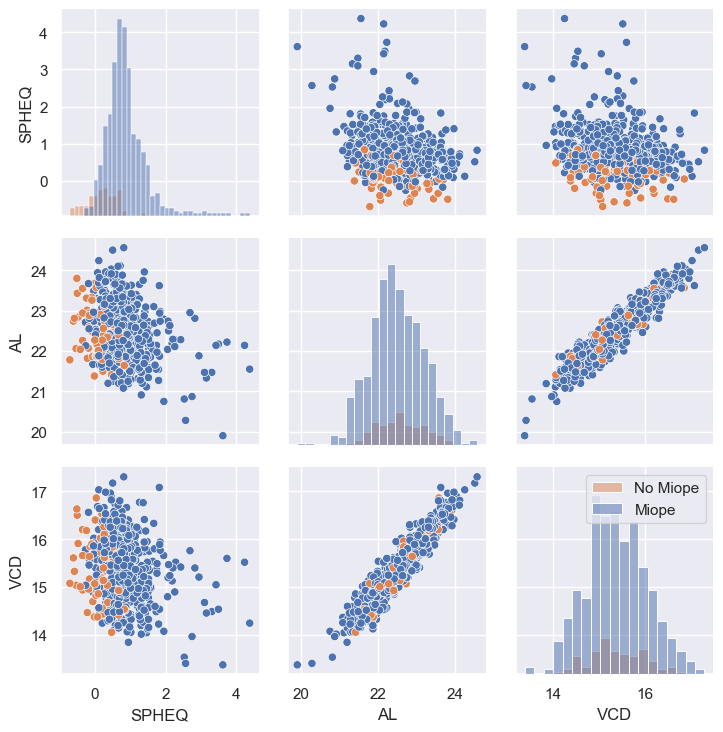
\includegraphics[height = .75\linewidth, width=.8\linewidth]{assets/focused_pairplot}
		\end{center}
		\caption{Gráfico por pares de las variables AL, VCD, SPHEQ, y la presencia de miopía (puntos en naranja).}
		\label{fig:4}
	\end{figure}
	 
	 En  la Figura \ref{fig:1} puede notarse que la Longitud Axial en los datos parece estar normalmente distribuida, de ahí que se realicen análisis más rigurosos a esta variable para conocer qué posibles propiedades cumple.

	 \begin{figure}[htb]
		\begin{subfigure}{.49\linewidth}
			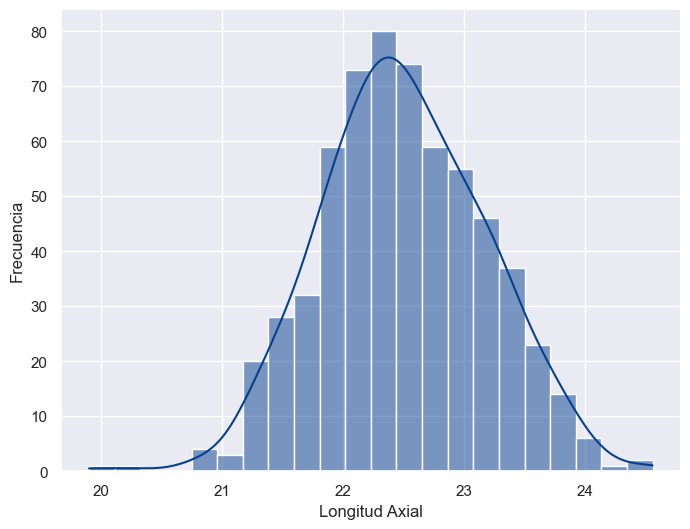
\includegraphics[height=.95\linewidth, width=.95\linewidth]{assets/AL_hist}
			\caption{}
			\label{fig:1a}
		\end{subfigure}
		\begin{subfigure}{.49\linewidth}
			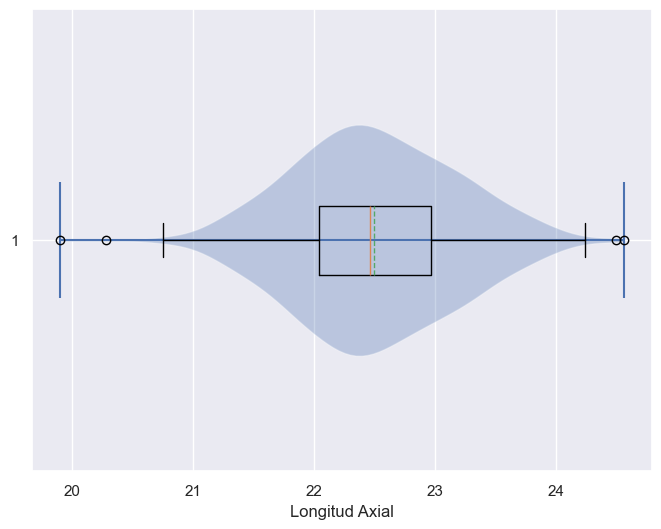
\includegraphics[height=.95\linewidth, width=.95\linewidth]{assets/AL_boxplot}
			\caption{}
			\label{fig:1b}
		\end{subfigure}
		\caption{La distribución de la Longitud Axial, representada en un histograma (a), y gráfico de cajas, bigotes, y violín (b).}
		\label{fig:1}
	\end{figure}
	
	Se procede a realizar un gráfico Cuantil-Cuantil como se muestra en la Figura \ref{fig:2}. Efectivamente, los cuantiles teóricos de una población normalmente distribuida coinciden con los cuantiles muestrales. Luego, se estiman la media y desviación estándar de la población ($\mu \approx 22.50$ y $\sigma \approx 0.69$), y se realiza una prueba de bondad de ajuste, Kolmogorov- Smirnov, entre la muestra y una población normal teórica construida con los parámetros estimados previamente; arrojando \emph{p-value} $ = 0.77 > \alpha = 0.05$, donde $\alpha$ es el nivel de significancia. Por tanto, no se tiene evidencia suficiente para rechazar  la normalidad de la Longitud Axial.
	\\
	
		\begin{figure}[htb]%
		\begin{center}
			\centering
			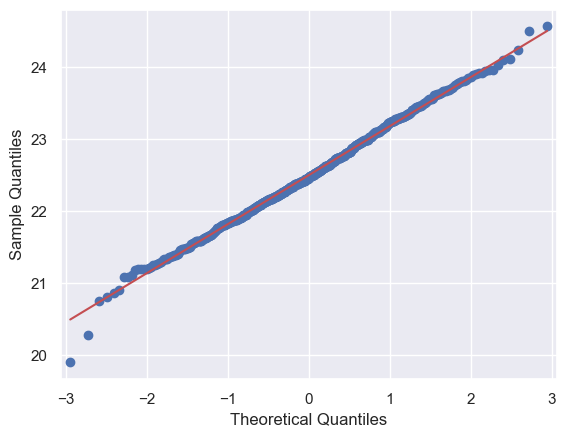
\includegraphics[height = .75\linewidth, width=.75\linewidth]{assets/AL_qqplot}
		\end{center}
		\caption{Gráfico Cuantil-Cuantil de la Longitud Axial, donde los cuantiles teóricos se refieren a una población normalmente distribuida.}
		\label{fig:2}
	\end{figure}
	
	 Los infantes suelen tener longitudes axiales uniformes cuando son muy pequeños, pero después de los 9 años, los niños tienden a mostrar longitudes axiales más largas que las niñas. Tiende, además, a diferenciarse según la etnia: los ojos asiáticos tienden a ser más largos que los ojos caucásicos, por ejemplo.
	 
	 En 2021 He X., Sankaridurg P. y un colectivo de científicos analizaron la correlación entre la AL en diferentes grupos etarios y la aparición de miopía en un estudio transversal en China. Dicho estudio incluyó un total de $14127$ participantes (en su mayoría chinos), y de ellos 5742 niños entre 7 y 10 años \cite{hex}. Entre sus resultados determinaron la media de la AL, con un valor aproximado de $22.9$ para un rango de edades similar al de la muestra bajo el presente análisis.
	 
	 De la estimación anteriormente calculada de la media muestral ($\bar{X} = 22.5 $). Luego, se comprueba mediante una prueba de hipótesis t-student si $H_0$: la media de la población de la que fue extraída la muestra coincide con la analizada por He X., $H_1$: la media de la población es menor. El resultado arrojó un $p-value = 1.22e-42 < \alpha$, por tanto se rechaza la hipótesis nula; se concluye que la población de nuestra muestra tiene una media significativamente menor. Del resultado anterior pruede comprobarse que efectivamente los ojos de niños caucásicos tienen una AL significativamente menor a los de asiáticos (al menos provenientes de China), aunque se debe tener en cuenta la brecha temporal entre ambos estudios.

	Se comprueba, además, que la nuestros datos fueron extraídos de una población con media $\mu \in [22.44, 22.55]$ con un $95\%$ de confianza, asumiendo que se desconoce la varianza población (por tanto calculando el intervalo de confianza con el estadígrafo \emph{t}).
	
%-----------------------------------------------------------------------------------
\subsection{Análisis de Varianza}\label{sub:anova}
%-----------------------------------------------------------------------------------
	La herencia genética así como factores anatómicos como la Longitud Axial, como ya se ha visto, juega un papel importante en la determinación de la Miopía en los pacientes, por tanto se propone analizar como afecta la herencia en esta característica particular en la decendencia. Se proponen dos enfoques al análisis de varianza ANOVA: primero para determinar si la herencia es significativamente determinante en la proporción de la Logitud Axial; y, más especificamente, si la herencia por parte de la madre o el padre (incluso ambos o ninguno), es determinante, en la característica en cuestión.
	
	\subsubsection{Primer acercamiento}
		Se asume la herencia no sexual, es decir, se analizarán si las caracteristicas de la \emph{AL} están influenciadas por la miopía en la madre y el padre, como factores uniformemente determinantes. Esto particiona la muestra en tres grupos de interés:
		
		\begin{enumerate}
			\item Pacientes sin progenitores miopes.
			\item Pacientes con un solo progenitor miope.
			\item Pacientes con dos progenitores miopes.
		\end{enumerate}
		
	\subsubsection{Segundo acercamiento}
		Sin la asumción de la herencia no sexual se analiza como varia la \emph{AL} teniendo en cuenta si es padre es miope, si la madre los es, si ambos lo son, o ninguno, como grupos mutuamente excluyentes. De esta forma los grupos de interés son:
		
		\begin{enumerate}
			\item Pacientes sin progenitores miopes.
			\item Pacientes con padre miope solamente.
			\item Pacientes con madre miope solamente.
			\item Pacientes con ambos progenitores miopes.
		\end{enumerate}
	
	
		En para los dos enfoques, los resultados fueron similares \emph{p-values} $> \alpha = 0.05 $ ($0.80$ y $0.70$ respectivamente), por tanto no existe evidencia suficiente en los datos para afirmar que la herencia es significativamente influyente en la Longitud Axial de la decendencia. Esté resultado puede observarse en la Figura \ref{fig:3}, notése que entre las curvas de cada color no existe diferencia notoria en su forma y posición. Se comprueba además, el cumplimiento los supuestos de ANOVA: normalidad, homocedastisidad e independencia de las muestras. 
		
		\begin{figure}[htb]%
			\begin{center}
				\centering
				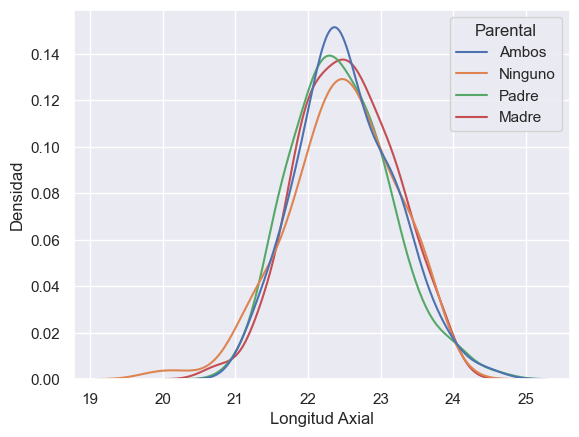
\includegraphics[height = .75\linewidth, width=.75\linewidth]{assets/AL_groups_kde}
			\end{center}
			\caption{Gráfico de Estimación de Densidad del Kernel (KDE por sus siglas en inglés), para cada grupo según su información parental.}
			\label{fig:3}
		\end{figure}
	
	
%-----------------------------------------------------------------------------------
%	\subsection{Listas y Descripciones}\label{sub:lists}
%%-----------------------------------------------------------------------------------
%		Para producir listas enumeradas, utilice el siguiente estilo:
%		\begin{enumerate}
%			\item Primer Elemento
%			\item Segundo Elemento
%			%
%			\begin {enumerate}
%				\item {Segundo Elemento - Subítem Uno}
%				\item {Segundo Elemento - Subítem Dos}
%			\end {enumerate}
%			%
%		\end{enumerate}
%
%%-----------------------------------------------------------------------------------
%		Para producir descripciones, use el siguiente estilo:
%
%%-----------------------------------------------------------------------------------
%		\begin{description}
%			\item [Primer Elemento] con su respectiva descripción.
%			\item [Segundo Elemento] también con su respectiva descripción.
%		\end{description}


%%-----------------------------------------------------------------------------------
%	\subsection{Código Fuente}\label{sub:listings}
%%-----------------------------------------------------------------------------------
%		Para producir código fuente, envuélvalo en una figura flotante y
%		etiquételo correctamente. Por ejemplo, en la Fig. \ref{fig:code}
%		se muestra un código bastante conocido\ldots
%
%		% Configuración de Listings
%		\lstset{keywordstyle=\color{blue}, basicstyle=\small}
%
%		\begin{figure}[htb]%
%			\begin{lstlisting}[language=c]%
%
%    int main(int argc, char** argv)
%    {
%        // Imprimiendo "Hola Mundo".
%        printf("Hello, World");
%    }
%
%			\end{lstlisting}
%		\caption{Código fuente de ejemplo.\label{fig:code}}
%		\end{figure}

%%-----------------------------------------------------------------------------------
%	\subsection{Referencias}
%%-----------------------------------------------------------------------------------
%  	Las referencias deben estar agrupadas en una sección al final del artículo,
%  	y las citas numeradas correctamente, por ejemplo \cite{knuth} o \cite{goedel}.
%  	Incluya toda la información importante de cada referencia, incluídos autor,
%  	título, y notas de la edición. En caso de citar sitios web, además
%  	de la URL, incluya la fecha en que fue consultado, como en \cite{wiki}. Numere 
%  	las referencias según el orden en que se les cita.

%===================================================================================



%===================================================================================
% Conclusiones
%-----------------------------------------------------------------------------------
\section{Conclusiones}\label{sec:conc}

  Se probó que, aunque el factor genético pueda influenciar la miopía, no existe evidencia suficiente que la presencia de la enfermedad en los padres influencia notoriamente en la anatomía de los ojos de la decendencia a tempranas edades. Se comprobó además que la AL sigue una distribución normal, y que efectivamente factores étnicos son definitorios en el tamaño del globo ocular, y por tanto puede ser determinante en el riesgo de aparición de la enfermedad. Sentando con todos estos elementos, las bases para un posterior análisis predictivo de la enfermedad a edades tempranas.

%===================================================================================



%===================================================================================
% Recomendaciones
%-----------------------------------------------------------------------------------
\section{Recomendaciones}\label{sec:rec}

 Probadas las capacidades de las herramientas convencionales para el análisis de datos en este campo tan importante de la medicina, se recomienda realizar un estudio mas preciso sobre la Miopía en Cuba, teniendo en cuenta los factores étnicos que componen su sociedad. Debe tenerse en cuenta que la cantidad de pacientes diagnosticados con miopía, a pesar de ser lo suficientemente grande para plantear pruebas de hipótesis, es considerablemente baja teniendo en cuenta los pacientes emétropes; lo cual puede afectar cosiderablemente la precisión de cualquier modelo predictivo que se formule con los datos, siendo estos propensos a errores de tipo 2, falsos negativos, diagnóstico erróneo en pacientes enfermos.

%===================================================================================



%===================================================================================
% Bibliografía
%-----------------------------------------------------------------------------------
\begin{thebibliography}{99}
%-----------------------------------------------------------------------------------
	\bibitem{semi} Sociedad Española de Medicina Interna (SEMI). URL: \href{https://www.fesemi.org/informacion-pacientes/conozca-mejor-su-enfermedad/miopia}
	{https://www.fesemi.org}.
	Consultado en \today.
	
	\bibitem{kaggle} Kaggle: Myopic risk comparison. URL:
	\href{https://www.kaggle.com/code/maryanalyze/myopia-risk-compare-lr-ebm-gbdt-model-performance}
		{http://www.kaggle.com}
		
	\bibitem{zadnikpredictors} Zadnik, K., Mutti, D. O., Friedman, N. E., Qualley, P. A., Jones, L.A., Qui, P., Kim, H. S., Hsu, J. C., \& Moeschberger, M. L. (1999). \emph{Ocular predictors of the onset of juvenile myopia. Investigative ophthalmology \& visual science}, 40(9), 1936–1943. \href{https://pubmed.ncbi.nlm.nih.gov/10440246/}.

	\bibitem{hex} He X, Sankaridurg P, Naduvilath T, Wang J, Xiong S, Weng R, Du L, Chen J, Zou H, Xu X. \emph{Normative data and percentile curves for axial length and axial length/corneal curvature in Chinese children and adolescents aged 4-18 years.} Br J Ophthalmol. 2023 Feb;107(2):167-175. doi: 10.1136/bjophthalmol-2021-319431. Epub 2021 Sep 16. PMID: 34531198; PMCID: PMC9887397.
	
	
%	\bibitem{knuth} Donald E. Knuth. \emph{The Art of Computer Programming}.
%		Volume 1: Fundamental Algorithms (3rd~edition), 1997.
%		Addison-Wesley Professional.
%
%	\bibitem{goedel} Kurt Göedel. \emph{Über formal unentscheidbare Sätze der
%		Principia Mathematica und verwandter Systeme, I}.
%		Monatshefte für Mathematik und Physik 38.
%
%	\bibitem{wiki} Wikipedia. URL: \href{http://en.wikipedia.org}
%	  {http://en.wikipedia.org}.
%		Consultado en \today.

%-----------------------------------------------------------------------------------
\end{thebibliography}

%-----------------------------------------------------------------------------------

\label{end}

\end{document}

%===================================================================================
